\begin{center}
\section{Stima del magnetone di Bohr $\mu_B$}
\end{center}
\medskip
{\color{gray}\hrule}
\medskip
Dalla teoria dell’interferometro di Fabry--Perot è possibile correlare la
separazione radiale delle frange osservate con la differenza in numero d’onda $k$ tra due
componenti spettrali.
Si ottiene

\[
\Delta k = \frac{1}{2 \mu t}\,\frac{\delta}{\Delta},
\]

dove $\mu=1.4560$ (per $\lambda\approx643$nm) è l’indice di rifrazione dell'\textit{etalon}
interno all’interferometro e $t=3$mm il suo spessore.\\
Combinando tale relazione con l’espressione dello splitting Zeeman 
$$\Delta E = \Delta m_lg\mu_BB$$
si ottiene
\[
\frac{\delta}{\Delta} = \frac{2 g \mu t \mu_B}{hc}\, B\Delta m_l .
\]
Nel caso dell’effetto Zeeman normale si ha $g=1$, dunque la relazione precedente è lineare:
$$\frac{\delta}{\Delta} = b\, B$$
Si interpolano dunque i dati sperimentali mediante una regressione lineare:
\[
\frac{\delta}{\Delta} = a + b\,B ,
\]
dove $a$ rappresenta l'intercetta e $b$ il coefficiente angolare della retta. \\
Dal valore del coefficiente angolare si ricava il magnetone di Bohr, invertendo
la relazione precedente:
\[
\mu_B = \frac{hc}{2 \mu t}\, |b| .
\]
\textit{Osservazione} Per i dati presi in configurazione longitudinale, questa stima va
ulteriormente divisa per un fattore 2, poiché la differenza energetica tra le righe considerate è
due volte quella dello splitting Zeeman.
\subsection{Geometria longitudinale}
Le coppie di dati $\left(B(I),\frac{\langle\delta\rangle}{\langle\Delta\rangle}\right)$, dove i valori di $B$ sono stati calcolati a partire dalle misure di corrente $I$ usando la relazione \ref{eq:cal_magn}, per la geometria longitudinale (riportati in appendice \ref{sec:longit}) seguono un andamento lineare.
\begin{figure}[H]
    \centering
    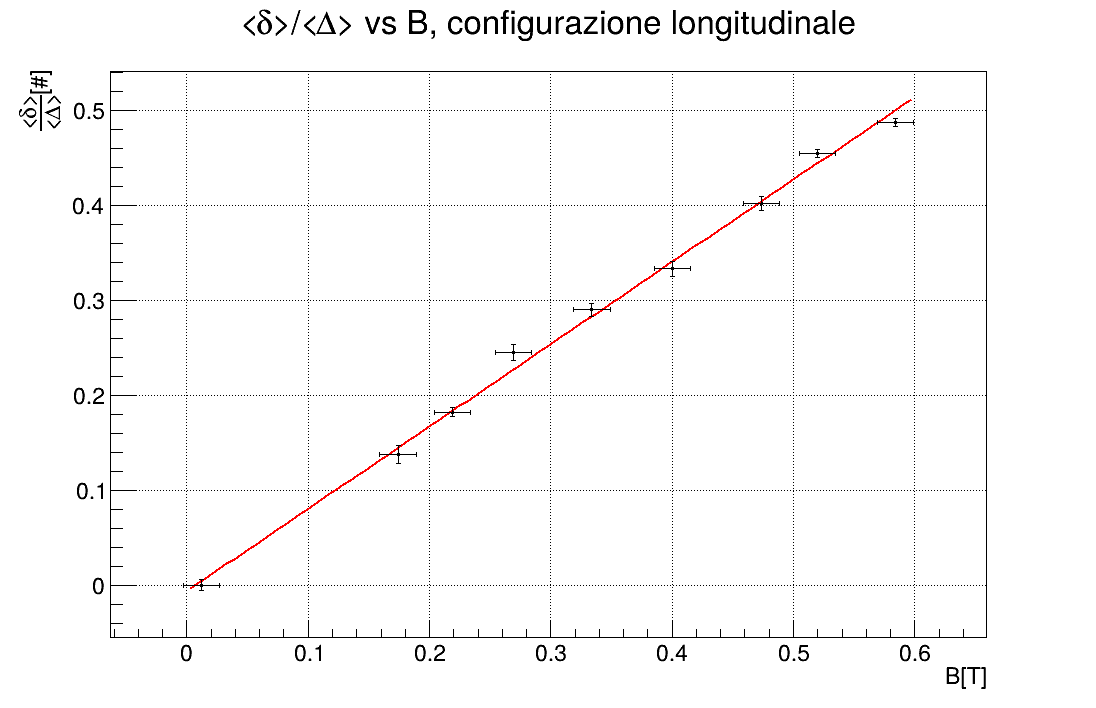
\includegraphics[width=.8\linewidth]{longit/longit.png}
    \caption{\footnotesize Coppie di dati $\left(B,\frac{\langle\delta\rangle}{\langle\Delta\rangle}\right)$, con regressione lineare $y=a+bx$ con parametri
    $a=-0.006\pm0.010$, 
    $b=(0.87\pm0.03)\text{T}^{-1}$,
    $\chi^2=3.5$ e d.o.f.$=7$.}
\end{figure}
Il termine noto risulta statisticamente compatibile con 0, come previsto dalla teoria, mentre dal
coefficiente angolare si ricava la stima
$$\mu_{B,l} = (9.9\pm0.3)\cdot10^{-24} \text{JT}^{-1}
$$
che risulta statisticamente compatibile con il valore teorico
$$
\mu_{B,th} = \frac{e\hbar}{2m_e} = 9.270100657(29) \cdot10^{-24}\text{JT}^{-1}
$$
\subsection{Geometria trasversale}
Entrambi i set di dati $\left(B,\frac{\langle\delta\rangle}{\langle\Delta\rangle}\right)$ per la
geometria trasversale (riportati in appendice \ref{sec:trasv}) seguono un andamento lineare:
il coefficiente angolare avrà lo stesso segno di $\Delta m_l$, in quanto questo è il segno di
$\Delta E$.
\begin{multicols}{2}
\begin{figure}[H]
    \centering
    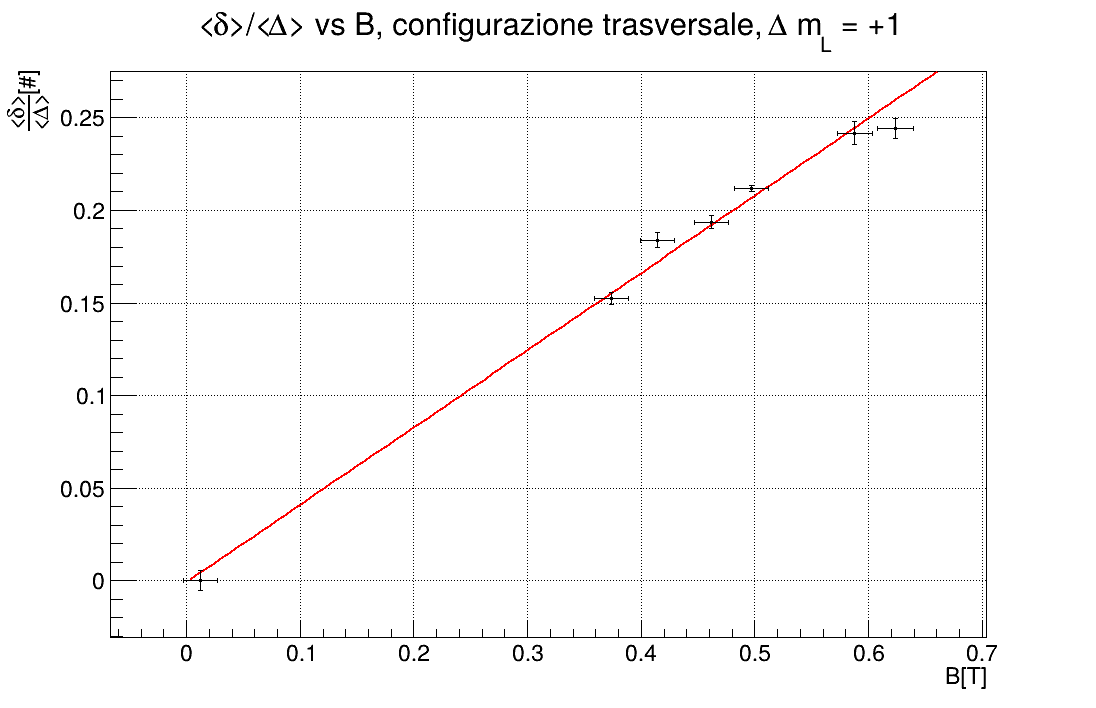
\includegraphics[width=\linewidth]{trasv/trasv_up.png}
    \caption{\footnotesize Coppie di dati $\left(B,\frac{\langle\delta\rangle}{\langle\Delta\rangle}\right)$, con regressione lineare $y=a+bx$ con parametri
    $a=-0.0007\pm0.0080$, 
    $b=(0.417\pm0.017)\text{T}^{-1}$,
    $\chi^2=6.8$ e d.o.f.$=5$.}
\end{figure}
\begin{figure}[H]
    \centering
    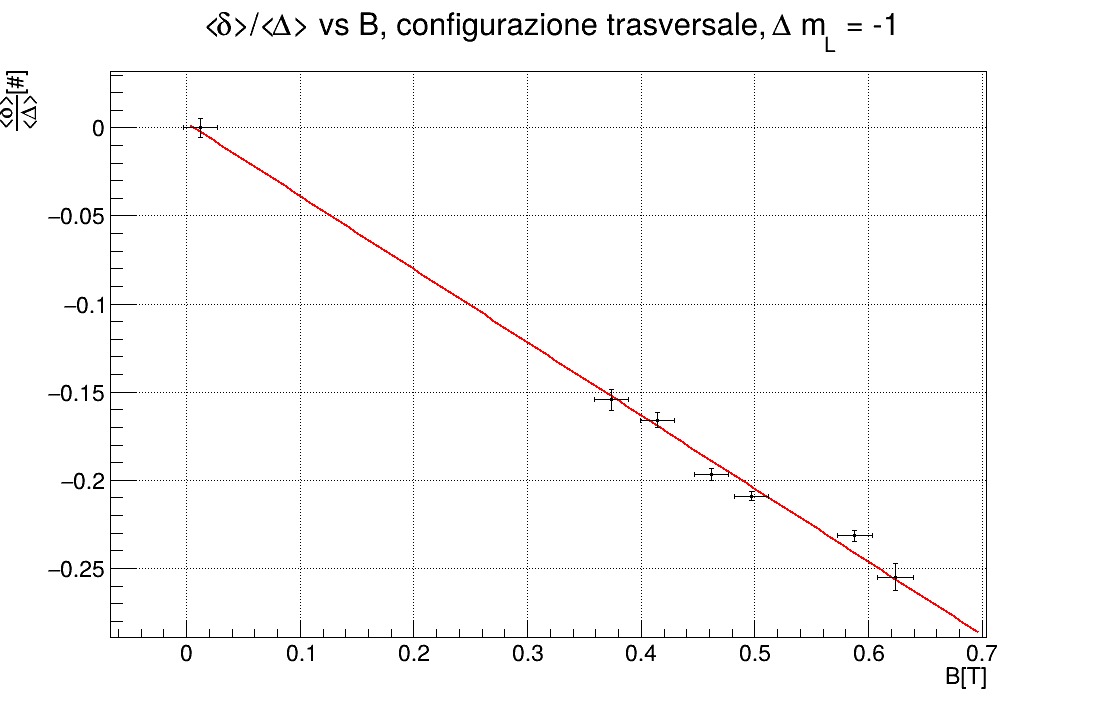
\includegraphics[width=\linewidth]{trasv/trasv_down.png}
    \caption{\footnotesize Coppie di dati $\left(B,\frac{\langle\delta\rangle}{\langle\Delta\rangle}\right)$, con regressione lineare $y=a+bx$ con parametri
    $a=0.003\pm0.008$, 
    $b=(-0.415\pm0.017)\text{T}^{-1}$,
    $\chi^2=4.2$ e d.o.f.$=5$.}
\end{figure}
\end{multicols}
In entrambe le regressioni il termine noto risulta compatibile con 0, come previsto dalla teoria,
mentre dai coefficienti angolari si ricavano le due stime
\begin{gather*}
    \mu_{B,t1} = (9.5\pm0.4)\cdot10^{-24}\text{JT}^{-1}\\
    \mu_{B,t2} = (9.4\pm0.4)\cdot10^{-24}\text{JT}^{-1}
\end{gather*}
che risultano entrambe compatibili con il valore atteso teorico.

Le tre stime di $\mu_B$ sono inoltre statisticamente compatibili tra loro e la loro media pesata vale
$$\langle\mu_B\rangle =  (9.6\pm0.2)\cdot10^{-24}\text{JT}^{-1}$$
che è statisticamente compatibile con il valore teorico.
\newpage
